%%% The main file. It contains definitions of basic parameters and includes all other parts.

%% Settings for single-side (simplex) printing
% Margins: left 40mm, right 25mm, top and bottom 25mm
% (but beware, LaTeX adds 1in implicitly)
% \documentclass[12pt,a4paper]{report}
% \setlength\textwidth{145mm}
% \setlength\textheight{247mm}
% \setlength\oddsidemargin{15mm}
% \setlength\evensidemargin{15mm}
% \setlength\topmargin{0mm}
% \setlength\headsep{0mm}
% \setlength\headheight{0mm}
% % \openright makes the following text appear on a right-hand page
% \let\openright=\clearpage

%% Settings for two-sided (duplex) printing
\documentclass[12pt,a4paper,twoside,openright]{report}
\setlength\textwidth{145mm}
\setlength\textheight{247mm}
\setlength\oddsidemargin{14.2mm}
\setlength\evensidemargin{0mm}
\setlength\topmargin{0mm}
\setlength\headsep{0mm}
\setlength\headheight{0mm}
\let\openright=\cleardoublepage

%% Generate PDF/A-2u
\usepackage[a-2u]{pdfx}

%% Character encoding: usually latin2, cp1250 or utf8:
\usepackage[utf8]{inputenc}

%% Prefer Latin Modern fonts
\usepackage{lmodern}

%% Further useful packages (included in most LaTeX distributions)
\usepackage{amsmath}        % extensions for typesetting of math
\usepackage{amsfonts}       % math fonts
\usepackage{amsthm}         % theorems, definitions, etc.
\usepackage{bbding}         % various symbols (squares, asterisks, scissors, ...)
\usepackage{bm}             % boldface symbols (\bm)
\usepackage{graphicx}       % embedding of pictures
\usepackage{fancyvrb}       % improved verbatim environment
\usepackage{natbib}         % citation style AUTHOR (YEAR), or AUTHOR [NUMBER]
\usepackage[nottoc]{tocbibind} % makes sure that bibliography and the lists
			    % of figures/tables are included in the table
			    % of contents
\usepackage{dcolumn}        % improved alignment of table columns
\usepackage{booktabs}       % improved horizontal lines in tables
\usepackage{paralist}       % improved enumerate and itemize
\usepackage[usenames]{xcolor}  % typesetting in color
%\usepackage{epstopdf} 
\usepackage{mhchem} 
\usepackage{chemfig} 
\usepackage[obeyFinal]{easy-todo}
\usepackage[T1]{fontenc}
\usepackage[english]{babel}
\usepackage{subfig}
%\usepackage{titlesec}  % possible modifications of sections/titles typesetting


%% some hyphenation patterns
\hyphenation{char-ged phos-pha-ti-dyl-eth-an-ol-a-mi-ne phos-pha-ti-dyl-se-ri-ne}
\tolerance=2000


%%% Basic information on the thesis

% Thesis title in English (exactly as in the formal assignment)
\def\ThesisTitle{Simulation of processes in cellular membranes}

% Author of the thesis
\def\ThesisAuthor{Josef Melcr}

% Year when the thesis is submitted
\def\YearSubmitted{2018}

% Name of the department or institute, where the work was officially assigned
% (according to the Organizational Structure of MFF UK in English,
% or a full name of a department outside MFF)
\def\Department{Institute of Organic Chemistry and Biochemistry v.v.i., AS CR}

% Is it a department (katedra), or an institute (ústav)?
\def\DeptType{Institute}

% Thesis supervisor: name, surname and titles
\def\Supervisor{prof. Pavel Jungwirth}

% Supervisor's department (again according to Organizational structure of MFF)
\def\SupervisorsDepartment{Department of physical and macromolecular chemistry}

% Study programme and specialization
\def\StudyProgramme{Physics}
\def\StudyBranch{Biophysics, chemical and macromolecular physics}

% An optional dedication: you can thank whomever you wish (your supervisor,
% consultant, a person who lent the software, etc.)
\def\Dedication{%
\begin{quotation}
“It’s a dangerous business, Frodo, going out of your door,” he used to say. 
“You step into the Road, and if you don’t keep your feet, there is no telling where you might be swept off to.”
(J. R. R. Tolkien)
\end{quotation}

\begin{center}
To all people, who helped us on this adventurous journey.
\end{center}

\begin{figure}[h!] 
  \centering 
  \includegraphics[width=12 cm]{../img/dedication.pdf}
\end{figure} 

I am grateful to you for all you have done for me. 
I especially thank to my Ph.D. advisor Pavel Jungwirth 
for the amazing period of my life full of exciting science,
and for the great support to my scientific carrier as well as our family life. 
I cannot express enough gratitude to my wife Ad{\'e}la and to our two daughters Dorotka a Hermínka,
who fuelled me with love, vigour and happines. 
My special thanks belong to our families for their immense support and encouragement. 


}

% Abstract (recommended length around 80-200 words; this is not a copy of your thesis assignment!)
\def\Abstract{%
Many important processes in cells involve ions, e.g., 
fusion of synaptic vesicles with neuronal cell membranes 
is controlled by a divalent cation \ce{Ca^{2+}};
and the exchange of \ce{Na^+} and \ce{K^+}
drives the the fast electrical signal transmittion in neurons. 
We have investigated model phospholipid membranes and their interactions 
with these biologically relevant ions. 
Using state-of-the-art molecular dynamics simulations,
we accurately quantified their respective affinites 
towards neutral and negatively charged phospholipid bilayers. 
In order to achieve that,
we developed a new model of phospholipids termed ECC-lipids,
which accounts for the electronic polarization
via the electronic continuum correction implemented as charge rescaling. 
Our simulations with this new force field 
reach for the first time a quantitative agreement 
with the experimental lipid electrometer concept 
for POPC as well as for POPS with all the studied cations. 
We have also examined the effects of transmembrane voltage on phospholipid bilayers. 
The electric field induced by the voltage 
exists exclusively in the hydrophobic region of the membrane,
where it has an almost constant strength. 
This field affects the structure of nearby water molecules 
highligting its importance in electroporation. 
}

% 3 to 5 keywords (recommended), each enclosed in curly braces
\def\Keywords{%
 {molecular dynamics simulations}, {molecular modeling}, {polarizability},
{biological membranes}, {phospholipid bilayers}, {phosphatidylcholine}
{transmembrane potential},
{sodium}, {potassium}, {calcium}
}

%% The hyperref package for clickable links in PDF and also for storing
%% metadata to PDF (including the table of contents).
%% Most settings are pre-set by the pdfx package.
\hypersetup{unicode}
\hypersetup{breaklinks=true}

% Definitions of macros (see description inside)
\include{macros}

%%%%%%%%%%%%%%%%%%%%%%%%%%%%%%%%%%%%%%%
%%%%%%%%%%%%%%%%%%%%%%%%%%%%%%%%%%%%%%%
% Title page and various mandatory informational pages
\begin{document}

%%% Custom variables
% width suitable for fitting into a column in 1-column page layout
\newlength{\figwidth}
\setlength{\figwidth}{9 cm} 
\newlength{\figwidthsmall}
\setlength{\figwidthsmall}{6 cm} 
\newlength{\figwidthfull}
\setlength{\figwidthfull}{14 cm} 

%%%%%%%%%%%%%%%%%%%%%%%%%%%%%%%%%%%%%%%
\include{title}

%%% A page with automatically generated table of contents of the doctoral thesis

\tableofcontents

%%% Each chapter is kept in a separate file
\chapter*{Introduction}
\addcontentsline{toc}{chapter}{Introduction}

 \textbf{1-2 paragraphs about the main topic of the thesis.} 


\chapter{Biological membranes}

 Introduction to the field. 
 \cite{Student08}

 Phospholipids. 

 Interaction with cations -- significance. 

 What is known in this respect. 

 Contradiction between simulation/experimental studies 
(use what's in the paper PCCP NMRLipids II). 

Experimental studies. 

\section{NMR order parameter measurements}

\section{Electrometer concept}

\section{SAXS? + other techniques (just to make the lit. research complete) -- probably not.}


\chapter{Molecular modeling of biological membranes}
\label{chap:methods}

Biological membranes are of a great interest in biology and biophysics. 
The tools and methods that enable their research have greatly evolved over the last decades. 
Nowadays, there is a plethora of membrane models and experimental methods, 
each having its benefits and drawbacks \citep{REF} \todoi{1-2 chosen reviews, everything else in prev chapter}
(see section~\ref{sec:modelmemb} in chapter~\ref{chap:intro} for a detailed overview). 

Molecular simulation can be considered as one of the newer approaches in this field. 
Starting with simple membrane models \citep{REF} \todoi{REF: few old/new simulation works},
simulation of membranes has evolved into a field of computational biophysics
that is capable of answering fundamental questions.
The recent progress in computational resources and algorithms
has allowed the simulations to grow in spatial scales and composition complexity
bringing more relevance for applications in biology. \citep{REF: CECAM workshop} \todoi{REF to CECAM workshop 2018 Lugano}

Molecular dynamics simulations of biological membranes employ classical particle-based models of molecules. 
Vast majority of the models are built using classical non-polarizable particles, 
each representing an individual atom (atomistic models), 
or a group of atoms (united-atom or coarse grained models). 
The following classical models belong among the most popular in membrane modeling:
\begin{itemize}
 \item Atomistic
 \begin{itemize}
   \item CHARMM \citep{klauda10}
   \item Slipids \citep{jambeck12, jambeck12b}
   \item OPLS lipids by \citet{maciejewski14}
   \item Lipid14 \citep{dickson14}
  \end{itemize}

 \item Coarse grained
 \begin{itemize}
   \item MARTINI \citep{marrink07}
   \item Berger \citep{Berger97}
   \item CHARMM-UA \citep{lee14}
  \end{itemize}
\end{itemize}

Despite all successes and valuable insights simulations have provided, 
there is still a large room for possible improvements of the current simulation models. 
For example, recent studies by \citet{botan15, catte16} has shown 
that both structure and interaction of phospholipid models require further optimization 
in order to become capable of interpreting solid state NMR experiments. 
In particular, we have discovered that 
the lack of polarizability is a major issue in any of the models 
from the above mentioned works \citep{botan15, catte16}
when interactions with charged moieties become important. 
Several possible ways for embedding polarizability into simulations, both explicit and implicit, 
will be introduced in the following sections. 





\section{Classical molecular dynamics simulations}
\label{section:md}

Classical molecular dynamics simulation provides insight into the dynamics and structure of molecules. 
It is commonly used for generating equilibrium thermodynamic ensembles,
that cas serve as input for statistical methods to extract observable equilibrium quantities. 
Classical MD simulation can be also used to assess the evolution of non-equilibrium states.
Such application is commonly termed as \emph{Steered MD}. 
Molecular modeling, and MD simulation in particular, 
is often combined with experiments,
which helps in their interpretation and provides detailed insight. 

In a MD simulation, the system of interest is propagated numerically in discrete time steps.
Newton equations of motion are used for systems with calssical particles, which form the majority of applications.
Interactions between particles, which often represent individual atoms, 
are described by an approximate interaction potential, also called \emph{force field}. 

The form of the force field varies with the model potentials that are used for the description of the individual interaction components. 
As an example, the interaction potential of AMBER \citep{ferrer13}, a popular model for biomolecules, has the following form:
 % Amber potential energy form:
\begin{eqnarray}  \label{eq:amber}
  V = & \displaystyle \sum _{bonds} K_b (r-r_{0})^2 + \sum _{angles} K_\Theta (\Theta-\Theta_{0})^2 + \\ \nonumber
      & \displaystyle \sum _{dihedrals} \frac{1}{2} V_n (1+\cos(n\phi -\phi_0)) + \sum _{i<j} \left [ s_{ij} ^{VdW} \left( \frac{A_{ij}}{r_{ij} ^{12}} - \frac{B_{ij}}{r_{ij} ^6} \right ) + s_{ij}^q \frac{q_i q_j}{\epsilon \, r_{ij}} \right ]
\end{eqnarray}
The first three terms represent the intra-molecular forces arising from bond stretching, angle bending and dihedral angle torsion. 
The symbols $K$ and $V$ are the force constants that describe the strength of such an interaction,
$r$, $\Theta$ and $\phi$ are the respective dimensions,
and $n$ is the multiplicity of the torsion potential. 

The last terms in the square brackets represent the inter-molecular interactions; the dispersion, or Van der Waals forces, and electrostatic interaction. 
Depending on the model force field, the non-bonded interactions are evaluated only for atoms separated by more than three or four bonds, 
which is here formally introduced through the matrix $s_{ij}$ that modifies the interaction accordingly.

The constants in matrices $A_{ij}$ and $B_{ij}$ represent the strengths of the repulsion and attraction forces 
arising from disperion and the overlap of the electronic clouds of the individual particles.  
The electrostatic interaction is described by the interacting partial charges $q_i$ and by the formally applied dielectric constant $\epsilon$ of the medium, 
which is assumed to be 1 in most force fields for biomolecules. 
In a later section~\ref{section:ecc}, we will show how to modify this interaction 
by changing the dielectric constant $\epsilon$ to include the effects of electronic polarization. 

Note that the interactions are simplified not only by the empirical formulae for the individual contributions, 
but to a large extent also by assuming that the interaction potentials are \emph{pair-wise additive}. 
Especially in the case of the inter-molecular forces, this is a severe assumption, 
which neglects the contributions from three and higher-body interactions. 
It was, however, shown that even such an approximate interaction potential is sufficiently accurate in many cases 
(see the list in the beginning of this chapter for such examples). 

The electrostatic interaction yields the strongest inter-molecular forces. 
In classical MD simulation, the electrostatic interaction is approximated by point charges in the centres of the particles. 
It has non-negligable contributions even from long distances. 
In periodic systems, i.e. in simulations with periodic boundary conditions, 
evaluating contributions from all periodic images is necessary. 
In neutral systems, this is efficiently done by 
summing the long range contributions in Fourier space rather than in real space
using fast algorithms developed for this purpose. \citep{darden93, essman95}

The dispersion interaction in the example empirical interaction potential in Equation~\ref{eq:amber} adopts the form of Lennard-Jones potential, 
which can be also expressed in terms of interaction energy $\epsilon_{ij}$ and the distance of the potential minimum, $\sigma_{ij}$, as
\begin{equation}
   U_{LJ} =  \frac{A_{ij}}{r_{ij}^{12}} - \frac{B_{ij}}{r_{ij}^6} = \epsilon _{ij} \left [ \left (\frac{\sigma _{ij}}{r_{ij}} \right )^{12} - 2 \left ( \frac{\sigma _{ij}}{r_{ij}} \right )^6 \right ] .
\end{equation}
The parameter $\sigma$ separates the regions, 
where the interaction is repulsive (distances smaller than $\sigma$), 
and where they are attractive (distances larger than $\sigma$). 
Such a parameter hence also tells on the size of the spherical particle, 
which has an impact on the balance between electrostatic and Van der Waals forces.

The parameters $\sigma_{ij}$ and $\epsilon_{ij}$ are usually derived for a small set of pairs,
and the parameters for any other pair of particles are derived by using combination formulae. 
The most common combination rules are Lorentz-Berthelot's:
\begin{equation}
 \sigma _{ij} = \frac{1}{2} (\sigma _{ii} + \sigma _{jj}) \, ; \quad \epsilon _{ij} = \sqrt{\epsilon _{ii} \, \epsilon _{jj}} 
\end{equation}









\section{Including polarizability}

\todo{This section can be included-or-omitted at leisure.}
The lack of electronic polarizability in standard MD simulation
force fields has been considered a serious issue since the early days of
lipid bilayer simulations \dots
  Lit. research (history) on how people include polarizability in classical simulations. 

\subsection{Explicit treatment of electronic polarizability}

\todo{This section can be included-or-omitted at leisure.}
 Joint subsection on Drude particles and polarizable dipoles, the most common ways of introducing polarizability explicitly into the MD simulation. 
\ldots rather demanding explicit inclusion
of electronic polarization effects \cite{lucas12,chowdhary13} \dots





\subsection{Electronic continuum correction as implicit treatment of electronic polarizability}
\label{section:ecc}

The theory for accounting for electronic polarization in empirical force fields
was originally developed by \citet{leontyev09} under the name Molecular Dynamics in Electronic Continuum, MDEC. 
The term Electronic continuum correction, ECC, originates in the works by \citet{Pluharova2014, kohagen14, kohagen16, martinek17},
where the rigorously developed theory from \citep{leontyev14} was applied on ionic solutions.
Through the comparison of neutron scattering and/or \emph{ab-initio} data with classical MD simulations, 
the authors developed an array of models for cations an anions, here termed ECC-ions,
that embedded ECC as an implicit model polarizability for electrons. 

\todo{Extensions of this section are relatively easy and possible by incorporating more equations and MDEC theory.}

Electronic continuum correction (ECC) is an implicit model of electronic polarization. 
in which a system of polarizable particles is represented
with an equivalent system of particles with fixed charges
including the effects of electronic polarization \emph{implicitly} in a mean-field way. \citep{leontyev09, leontyev10, leontyev11, leontyev14}
This can be done by a relatively simple transform of the partial charges,
which does not change the form of the formula of the empirical force field (examples in section~\ref{section:md})
making a wrong impression of a \emph{non-polarizable} model again. 
Technically, ECC is similar to the phenomenological scaling of partial charges, 
which was applied in earlier studies of aqueous solutions or ionic liquids \citep{jonsson86,egberts94,beichel14},
in which also other possible effects (e.g. charge transfer) were considered.
In contrast, ECC is a physically well justified and rigorously derived model~\citep{leontyev09, leontyev10, leontyev11, leontyev14}.
The relation for the charges employing ECC model can be formally written as
\begin{equation}  \label{eq:scaling}
 Q^{ECC} = f_q \cdot Q ,
\end{equation} 
where $Q$ and $Q^{ECC}$ are the original and the scaled, \emph{implicitly polarized}, partial charges respectively. 
The relation between the original and the new set of charges 
is, hence, a mere linear scaling with a certain factor, $f_q$, 
which is related to the high-frequency dielectric constant, $\epsilon _{el}$, of the electrons according to
\begin{equation}   \label{eq:scaling_factor}
 f_q = \sqrt{ \epsilon _{el} }
\end{equation} 

The presented Relation~\ref{eq:scaling} is rather a practical way of implementing the ECC polarizability model into the simulation. 
It is equivalent to embedding all atoms into a dielectric continuum 
with the high-frequency dielectric constant of the electrons, $\epsilon _{el}$, providing the same effect.
It is important to note that the value of the high frequency dielectric constant  
is around 2 for almost any biologically relevant environment \citep{leontyev11}. 
This means that even interfaces like biological membranes do not contain discontinuities of the electronic continuum. 
The dielectric discontinuity in a lipid bilayer thus arises only 
from the orientational polarization of the molecules, which is accounted for explicitly in standard MD simulations.  
Therefore, the same correction for the electronic polarizability can be  
applied throughout the lipid bilayer/aqueous solution interface. 
Given that the  high frequency dielectric constant of water is 1.78 (i.e., the square of the refraction index), 
the scaling factor for ions in water is $\approx 0.75$. 





 

 
 



\section{Implicitly polarizable classical MD models of lipids using ECC}
\label{section:ecc-lipids}

Simulations with explicitly polarizable models are generally considered to be computationally too demanding for a practical use in biophysics. 
The models employing ECC, however, are on the same level with classical non-polarizable models with fixed charges, yet they implicitly incorporate electronic polarization. 
The ECC theory was introduced in the above section~\ref{section:ecc}.
In this section, I will demostrate the application of the ECC theory on phospholipids, 
where the effects of polarization yield crucial consequences in the accuracy of the interaction with ions. 

We chose phosphatidylcholine (PC), phosphatidylethanolamine (PE) and phosphatidylserine (PS)
as representants of the most common neutral and negatively charged lipids in plasma membrane \citep{the_review_with_pie_charts_on_my_desk, marsh13}. 
The Lipid14~\citep{dickson14} model was used for POPE and POPC,
and the Lipid17~\citep{lipid17} model, already available from AmberTools \citep{ferrer13},
were used as the starting point for embedding ECC.
It was shown by \citet{botan15, catte16} that such a family of lipid models provides one of the most 
realistic descriptions of the head group order parameters of POPC and their response to ions 
when compared to other available lipid models. 

In the case of POPS, which bears a total negative charge of -1, 
embedding ECC through the linear transform of the partial charges is straightforward. 
The resulting ECC-lipid model of POPS, also denoted as ECC-POPS, 
adopts a formal total charge $-0.75$ in line with ECC and the electronic dielectric constant of water \citep{leontyev14}. 
Note that the formal charge is equal in size to the charges of monovalent ions developed with ECC \citep{Pluharova2014, kohagen14, kohagen16, martinek17}.

While the scaling factor of $f_q = 0.75$ is undoubtedly justified for molecules with a non-zero total charge like ions or POPS,
it is not \emph{a priori} clear what factor shall be used for neutral molecules, i.e. for POPE and POPC in our case.

The partial charges of particles forming molecules in simulations are not physical observables unlike the total charge. 
There is a variety of schemes for assigning partial charges to particles in molecules~\citep{Hu2007}. 
The restrained electrostatic potential method (RESP) is, however, the most common method used in biomolecules~\citep{RESP_paper, Singh1984, dickson14}. 
In practice, it is common that water molecules are included in the RESP calculations, 
and charges are subsequently refined to improve certain experimental observables. 
Although such tweaks do not affect the zero total charge for neutral molecules,
it naturally follows that the effects of electronic polarizability 
may to some extent be present even in standard force fields~\citep{RESP_paper, Singh1984, jorgensen96, ipolq2013, benavides17}. 
We thus conclude that the scaling factor, $f_q$, for partial charges in existing models of neutral molecules does not necessarily follow the relation \ref{eq:scaling_factor}.
It is expected instead, that the scaling factor may adopt a slightly higher value than 0.75. 

The ECC correction was applied on top of the Lipid14/Lipid17 models of POPC, POPE and POPS
by scaling the partial charges of all atoms except acyl tails, 
i.e. the polar parts in phospholipids, head group, glycerol backbone, and carbonyl regions. 
Such a choice was guided by the observed strength of interaction with cations. 
In contrast, the acyl chains do not come in direct contact with ions from the solution, 
and they are already highly optimized to provide a good description of the
hydrophobic part of lipid bilayers \cite{dickson14,ollila16}.
Compared to the acyl tails, the glycerol backbone and the head group regions of phospholipids 
require improvements in any available lipid model~\cite{botan15}.

We found that the optimal value for the scaling factor of partial charges of the neutral molecules from the Lipid14 force field \citep{dickson14}
is $f_q = 0.8$, which is indeed close to 0.75, 
the scaling factor for the ions in water. 
This value was found by comparing the results from the simulations with POPC to the experimental 
NMR data~\cite{akutsu81,altenbach84,scherer89} on the head group order parameter response to the bound charge.
Note that common empirical scaling factors for solutions of monovalent ions in water 
are 0.8 or even higher \citep{benavides17,skinner14,nacleps}.  
In contrast, modern force fields for ionic liquids often employ values around 0.6--0.65, 
which are on the other hand much lower than $\epsilon^{-1/2}_{el}$ \citep{holm14}.

Although scaling of the partial charges improved 
the head group order parameter response and ion binding affinity,
it at the same time has deteriorated certain membrane properties; 
namely the area per lipid generally decreased, often below the experimental values. 
The decrease of the area per lipid is observed to likely arise from a reduced hydration of the lipid head group region
as the polarity of the head group has overall decreased after scaling charges. 

We compensated this effect
by reducing the effective radii of atoms with the scaled charges.
This was explicitly done for POPC by changing the parameters $\sigma$ in the Lennard-Jones potential 
in a similar way as was done previously for the ECC-ions in solution \cite{kohagen14,kohagen16,Pluharova2014}.
Reducing the $\sigma$ parameters of the affected atoms by a factor of $f_\sigma = 0.89$
restored the area per molecule to the level very close to the experiment (Table~\ref{tab:apls}). 
Such optimized parameters $\sigma$ were then used for all ECC-lipids, i.e. also for ECC-POPE and ECC-POPS. 
In addition, the X-ray scattering form factors of POPC, POPE and POPS from simulations remained at a good agreement or even improved with the modifications 
(see Figs.~\ref{simVSexpNOions}, \ref{simVSexpNOions_POPS} and \ref{simVSexpNOions_POPE}). 








\subsection{Structural parameters of model membranes with ECC-lipids: Agreement with experiments} 
 
%%%%%%%%%%%%%%%%%%%%%%%%%%%%%%%%%%%%%%%%%%%%%%%%%%%%%%%%%%%%%%
% problem solved: NO line breaks in the caption!
\begin{figure}[tb!] 
  \centering 
  \includegraphics[width=8.2cm]{../img/ecc_popc/Order-parameters_form-factors_exp-L14-ECCL17_q80_sig89_POPC-struct.pdf} 
  \caption{ \label{simVSexpNOions} 
    Top: X-ray scattering form factors from simulations with the Lipid14 \citep{dickson14} and 
    the ECC-POPC models compared with experiments~\citep{kucerka11} at 303~K. 
    Middle: Order parameters of POPC head group, glycerol backbone and acyl chains  
    from simulations with the Lipid14 \citep{dickson14} and the ECC-POPC models 
    compared with experiments \citep{ferreira13} at 300~K. 
    The size of the markers for the head group order parameters correspond to 
    the error estimate $\pm 0.02$ for experiments \citep{botan15,ollila16}, 
    while the error estimate for simulations is $\pm 0.005$
    (Bayesian estimate of 95\% confidence interval \citep{scipy}).
    The size of the points for acyl chains are decreased by a factor of 3 to improve the clarity of the plot.
    Open/closed symbols are used for palmitoyl/oleoyl chains of POPC. 
    Bottom: The chemical structure of POPC and the labeling of the carbon segments. 
  }  
\end{figure} 


\begin{figure}[tb!] 
  \centering 
  \includegraphics[width=\figwidth]{../img/ecc_pope/Order-parameters_form-factors_exp-ECC-POPE.pdf}
  \caption{\label{simVSexpNOions_POPE} 
    X-ray scattering form factors from simulations with 
    the ECC-lipids model of POPE compared with experiments~\cite{kucerka11} at 313~K. 
    Order parameters of POPE head group, glycerol backbone and acyl chains  
    from simulations with the ECC-lipids model of POPE
    compared with experiments by \citet{gally81} (order parameters of glycerol backbone, labeled \emph{E. coli} membrane at~310\,K, ) 
    and by \citet{seelig76, seelig80} (order parameters $\alpha$ and $\beta$ from DPPE at~341\,K).
    Open/closed symbols are used for palmitoyl/oleoyl chains of POPE. 
  }  
\end{figure} 


\begin{figure}[tb!] 
  \centering 
  \includegraphics[width=\figwidth]{../img/ecc_pops/order_parameters_actual_pure-POPS.pdf} 
  \includegraphics[width=\figwidth]{../img/ecc_pops/l17/order_parameters_actual_pure-POPS.pdf} 
  \includegraphics[width=\figwidth]{../img/ecc_pops/form-f_l17-ecc-pops-exp_compar.pdf} 
  \includegraphics[width=\figwidth]{../img/ecc_pops/lipids_chemfig.pdf} 
  \caption{\label{simVSexpNOions_POPS} 
    X-ray scattering form factors from simulations with the Lipid17 \cite{lipid17-future} and 
    the ECC-POPS models compared with experiments~\cite{SDP-CHARMM36_comparison_paper_Samuli-knows} at 298~K. 
    Order parameters of POPS head group, glycerol backbone and acyl chains  
    from simulations with the Lipid17 \cite{lipid17-future} and the ECC-POPS models 
    compared with \emph{experiments at 300~K (check and change)} measured by Tiago Ferriera. 
    Open/closed symbols are used for palmitoyl/oleoyl chains of POPS. 
    The chemical structure of POPS and the labeling of the carbon segments. 
  }  
\end{figure} 
%%%%%%%%%%%%%%%%%%%%%%%%%%%%%%%%%%%%%%%%%%%%%%%%%%%%%%%%%%%%%%
 
\begin{table}[tb!] 
  \caption{Values of the area per lipid (APL) of POPC, POPE and POPS bilayers without additional ions. \label{tab:apls} 
  } 
  \begin{tabular}{l|c c} 
    \multicolumn{3}{c}{POPC} \\
    \hline 
    model          & APL (Å$^2$)   & Temperature (K) \\ 
    \hline 
    Lipid14 POPC                    & 65.1$\pm$ 0.6  &  300 \\ 
    Lipid14 POPC \citep{dickson14}  & 65.6$\pm$ 0.5  &  303 \\ 
    \hline 
    ECC-POPC                & 63.2$\pm$ 0.6  &  300       \\ 
    \hline 
    experiment (SDP model) \citep{kucerka11} & 64.3  &  303    \\ 
    \hline 
    \\
    \multicolumn{3}{c}{POPE} \\
    \hline 
    model          & APL (Å$^2$)   & Temperature (K) \\ 
    \hline 
    ECC-POPE                 & 56.7$\pm$ 0.8  &  298 \\ 
    \hline 
    experiment   \citep{parsegian89} & 56.6  &  310    \\ 
    experiment   \citep{rappolt03}   & 60--62 &  308--318  \\ 
    \hline 
    \\
    \multicolumn{3}{c}{POPS} \\
    \hline 
    model          & APL (Å$^2$)   & Temperature (K) \\ 
    \hline 
    Lipid17 POPS              & 53.5$\pm$ 0.8  &  298 \\ 
    \hline 
    ECC-POPS                & 60.3$\pm$ 0.6  &  298       \\ 
    \hline 
    experiment (SDP model) \cite{SDP-CHARMM36_comparison_paper_Samuli-knows} & 62.3  &  298    \\ 
    \hline 
  \end{tabular} 
\end{table} 
 
 
We checked X-ray scattering form factors and NMR order parameters 
in pure water without any ions (or only counter ions)
as the first step in assessment of the quality of the model. 
The experimental X-ray scattering form factors 
of a bilayer are well reproduced by all lipids in the presented ECC-lipids model 
(see Figs.~\ref{simVSexpNOions}, \ref{simVSexpNOions_POPS} and \ref{simVSexpNOions_POPE}). 

The area per lipid is often used as a relatively simple structural parameter telling on the bilayer properties and the packing of lipids. 
In experiments, modeling is used on top of the scattering factors to obtain it \citep{SDP-CHARMM36_comparison_paper_Samuli-knows}. 
In simulations, this property is easily extracted. 
We compare the values from experiments and simulations in Table~\ref{tab:apls}. 
The area per lipid of ECC-POPE agrees well with the experiment by \citet{parsegian89}, 
however, the other experiment reported in Table~\ref{tab:apls} is considerably larger in the same temperature range. 
\todo{Correct the following argument -- the simulation/experiments are at different temperatures!}
Finding a very similar result for area per lipid of POPE using two independent models (ECC-lipids and \citep{parsegian89})
raises doubts about the estimation of the property in the work by \citet{rappolt03}. 

The area per lipid of POPC in simulation with ECC-lipids model is smaller by $\approx$1Å 
than the experimental value derived from the SDP model \citep{SDP-CHARMM36_comparison_paper_Samuli-knows}. 
The values of the area per lipid of the ECC-POPC model vary slightly 
when simulated with different water models, however,
they are still close to the experiment. 

While the agreement between the scattering form factors 
from the simulation of a pure POPS bilayer and experiment 
are excellent (Fig.~\ref{simVSexpNOions_POPS}),
there is a non-negligable difference between the values of the area per lipid in Table~\ref{tab:apls}. 
Since both values are derived from the scattering form factors through modeling of the electron density of the bilayer,
we cannot decide, which of the value is more reliable. 
In general, we can conclude that the presented lipid models within ECC-lipids 
reproduce the experimental dimensions of the lipid bilayers 
with a comparable accuracy to other state-of-the-art lipid models~\citep{ollila16}. 
 
The head group and acyl chain order parameters of the lipids within ECC-lipids
are in general in a good agreement with the experimental values 
as shown in Figs.~\ref{simVSexpNOions}, \ref{simVSexpNOions_POPE},  and \ref{simVSexpNOions_POPS}. 
The acyl chain order parameters in particular are almost all within the experimental error bars.
The order parameters of the head groups are at a common accuracy of classical models of lipids \citep{botan15, catte16}. 

The head group order parameters $\alpha$ and $\beta$ are highly relevant for this work,
as they are being used in the electrometer concept (introduced in section~\ref{section:electrometer}). 
For POPC, the order parameter $\beta$ agrees well with the experiment, 
while the order parameter $\alpha$ is somewhat lower. 
In the case of POPS, the situation is a bit more complicated
compared to POPC as the order parameter $\alpha$ exhibits a notable forking (see Fig.~\ref{simVSexpNOions_POPS}).
One of the order parameters of the ECC-lipids model of POPS, $\alpha_1$, agrees well with the experiment, 
while the other, $\alpha_2$, adopts a higher value underestimating the experimentally reported forking. 
There is only one order parameter $\beta$ in POPS, 
which has a higher value closer to zero in the ECC-lipids model than in experiment. 
Such a feature suggests that the model overestimates the orientational freedom of its head group. 

To our knoweldge, there are no data on the order parameters in POPE. 
To get at least a rough estimate of the structure of PE head group from experiments, 
we can compare to either DPPE, which has palmitoyls in both acyl tails, and is measured at a different temperatrue~341\,K \citep{seelig76, seelig80};
or a mixture of PE lipids from the membrane of \emph{E. coli} at~310\,K, \citep{gally81}. 
Such data are used in Fig.~\ref{simVSexpNOions_POPE} to provide some esimates of the order parameters from related systems. 
 
 
 

\chapter{Interactions of ions with phospholipid membranes}
\label{chap:results}

Biological membranes naturally exist in a weak electrolytic solution of \ce{KCl} on the intracellular side, and of \ce{NaCl} on the extracellular side. 
The biological relevance of these ions reaches from relatively simple osmotic effects to the complex processes in neural signalling. 

Calcium is an important cation in biology, 
which takes part in many signalling pathways, e.g. triggering of the release of neurotransmitter in neurons,
and processes such as regulating cardiac rythm in heart. 
The interaction of \ce{Ca^{2+}} with phospholipid membranes has recieved attention recently from both experiments and simulations \citep{melcrova16, javanainen17}.

In the previous chapter, we presented new classical MD models of phospholipids,
which account for electrionic polarization via ECC (introduced in section~\ref{section:ecc}). 
It was demonstrated that such models, termed ECC-lipids, 
meet current accuracy standards in the field 
by comparing them with NMR order parameters and X-ray diffraction data (section~\ref{section:ecc-lipids}. 

In this chapter, we will provide detailed insight into the interactions of these ions with neutral and negatively charged model membranes,
namely with a POPC bilayer and with a negatively charged bilayer with a composition of 5~POPC:1~POPS. 
We employ our newly developed models of ions and phospholipids, 
ECC-ions \citep{martinek17, kohagen16, Pluharova2014} and ECC-lipids \citep{melcr18}, 
which excel any state-of-the-art model of ions or lipids in terms of lipid-ion interactions. 

First, we summarize the literature knowledge on the interactions of ions with membranes in experiments and simulations.
Then we demonstrate the outstanding accuracy of the newly developed model of POPC, ECC-POPC, 
in the responses of the head group order parameters.
The simulation study with a cationic surfactant 
validates ECC-POPC as an accurate model of the lipid electrometer concept observed in NMR experimnents. 
At last, we will provide detailed insight into the binding of cations to the neutral and negatively charged bilayers. 
We put extra stress on the interactions with \ce{Ca^{2+}}, 
for which we present the first simulation results that are in \emph{quantitative} agreement with experiments. \citep{catte16, melcr18}





\section{Binding of cations to phospholipid bilayers and lipid electrometer concept from experiments and simulations}
\label{section:electrometer_exp_sim} 

The response of the head group order parameters 
to a certain amount of bound charge in the bilayer 
was calibrated using monovalently charged surfactants in \citep{scherer89}. 
After such a calibration,
binding affinities of free cations can be estimated from the measured head group order parameter changes. \citep{scherer89}
This forms the lipid electrometer concept (introduced in section\ref{section:electrometer}),
which can be used to directly compare experimental measurements with MD simulations. 
We performed such a comparison for both neutral and negatively charged membranes with \ce{NaCl} and \ce{CaCl2} 
for a large array of MD simulations produced within NMRlipids open collaboration platfrom \citep{nmrlipids}. 
It was concluded  that the binding affinities of cations are overestimated in almost all models studied in~\citep{catte16} (Fig.~\ref{fig:catte16}) and \citep{nmrlipids_proj4}. 


The small head group order parameter response of a neutral POPC bilayer to \ce{NaCl} from the experiments by~\citet{seelig87} is captured by only a few models, 
namely Lipid14 \citep{dickson14}, Orange (see supplementary infromation in \citep{catte16}) and CHARMM36 \citep{klauda10}. 
However, the experimentally measured head group order parameter response to \ce{CaCl2} is captured only \emph{qualitatively} by the models. \citep{catte16}
In addition, none of the employed models in that study reproduces the order parameters without any salt concentration
within experimental error, indicating structural inaccuracies of varying severity in all of them~\citep{botan15}.
In summary, all models of a POPC bilayer examined in \citep{catte16} 
overestimate the response of head group order parameters and/or binding affinity of \ce{CaCl2} to such bilayers. 



\begin{figure}[tbp]
  \centering
  \includegraphics[width=\figwidthfull]{../img/OrderParameterIONSchanges.pdf}
  \caption{\label{fig:catte16}
    Changes of the head group order parameters $\beta$ (top row) and $\alpha$ (bottom row) 
    to increasing concentrations of \ce{NaCl} (left column) and \ce{CaCl2} (right column)
    Results from experiments 
    (DPPC from Ref.~\citep{akutsu81}, POPC from Ref.~\citep{altenbach84}) 
    are compared with simulations gathered through NMRlipids open collaboration platform \citep{nmrlipids} in the work by \citet{catte16}. 
    Note that none of the employed models in this figure reproduces the order parameters without any salt concentration
    within experimental error, indicating structural inaccuracies of varying severity in all of them~\citep{botan15}.
  }
\end{figure}


Similar conclusions as for POPC bilayers are also found for 
negatively charged membranes with a composition 5\,PC:1\,PS in \citep{nmrlipids_proj4}. 
Although the structure of the lipids in a POPS bilayer with only \ce{Na^+} counterions
is again not captured within the experimental error bars,
the small response of the order parameters of PC and PS head groups 
to incresing concentrations of \ce{NaCl} in the mixed bilayer with a composition 5\,PC:1\,PS 
is maintained in a few models, 
namely Lipid17 \citep{lipid17-future} and less well in MacRog \citep{maciejewski14}. 
Interestingly, the response to \ce{CaCl2} is overestimated by all employed models but one, CHARMM36 obtained from \url{http://charmm-gui.org/} \citep{jo08, lee15},
which has incorporated a correction for the observed excessive binding of \ce{Ca^{2+}} to PC and PS similar to the correction for \ce{Na^+} \citep{venable13}. 
With such a model, the response of the head group order parameters of PC 
to increasing concentrations of \ce{CaCl2} in a mixed negatively charged bilayer
is significantly reduced by the employed correction for \ce{Ca^{2+}}
even below the response measured experimentally. 
Hence, it is the only model in the study,
which underestimates the response of the lipid electrometer for the negatively charged membrane
contrasting with the results from the neutral POPC bilayer in \citep{catte16}. 



\begin{figure}[tb!] 
  \centering 
  \includegraphics[width=\figwidth]{../img/ecc_popc/PN_angle_OrdPars-A-B_L14-ECCL17_q80_sig89_surf.pdf} 
  \caption{\label{OrderParameterCHANGESsurf} 
    The changes of head group order parameters and P-N vector orientation as a function of 
    a molar fraction of the cationic surfactant dihexadecyldimethylammonium in a POPC bilayer 
    from simulations and experiments \citep{scherer89} at 313 K.
  } 
\end{figure} 

 

In order to distinguish, whether the observed discrepancy of the head group order parameter changes between simulations and experiments 
arise from incorrect sensitivity of the head group or from mostly excessive binding of cations to the phospholipid bilayer,
we performed simulations of a neutral POPC bilayer with varying amounts of the cationic surfactant dihexadecyldimethylammonium, 
as was measured in the experimental work by \citet{scherer89}.
The amount of bound charge per PC 
in such systems is given simply by the molar fraction of the cationic surfactants, 
as essentially all of the surfactants locate to the lipid bilayers 
due to the two long hydrophobic tails.
The NMR measurements of such systems  
can be used to validate the sensitivity of lipid headgroup order parameters 
(i.e. the coefficient $m_i$ in Equation~\ref{OPchangeEQ}) 
to the amount of bound charge in simulations. 
The changes of the headgroup order parameters in a POPC bilayer with an increasing amount of 
the cationic surfactant from simulations and experiments~\citep{scherer89} are shown in Fig.~\ref{OrderParameterCHANGESsurf}.
In line with Equation~\ref{OPchangeEQ},
experiments and also both MD simulation models show approximately linear decrease of the head group order parameters $\alpha$ and $\beta$.

Results from simulations with two models are shown.
We employ our newly developed model ECC-POPC, introduced in the previous chapter, 
which accounts for electronic polarizability using ECC \citep{leontyev14}.
For a direct comparison, we also show results for Lipid14, a standard model by \citet{dickson14},
which served as a starting point in the development of ECC-POPC. 
This model was also used in the works \citep{catte16, nmrlipids_proj4}. 

While the slope of the response of order parameters $\alpha$ and $\beta$ 
from the simulation with ECC-POPC model 
is in a very good agreement with the experiments, 
the slope from Lipid14 is too steep
suggesting that the overestimated response observed also in \citep{catte16}
arises at least in part from an overly sensitive response of the head group. 

The increasing amount of cationic surfactant in the bilayer
also affects the P-N vector, 
which is defined as the angle between the connector of the phosphorus and nitrogen atoms and the membrane normal. 
Similarly to the order parameters, 
there is a linear dependence on the amount of the cationic surfactant
as shown in Fig.~\ref{OrderParameterCHANGESsurf}. 
Although the structure of ECC-POPC model without any ions does not agree with NMR experiments within errors,
such a model reproduces well the changes of the order parameters.
It follows that using this model,
we can write an approximate relation between the changes of the order parameters and the P-N vector mean orientation. 
For the change of the order parameter $\alpha$, $\Delta S^\alpha$, we arrive at
\begin{equation}
\Delta \vec{PN} = (186 \pm 9) \cdot \Delta S^\alpha .
\end{equation}

After reproducing the concept of a lipid electrometer with a known amount of bound surface charge,
ECC-lipids will be employed in the study of interactions with aquaeous ions, namely with \ce{K^+}, \ce{Na^+} and \ce{Ca^{2+}}. 












\section{Interactions of neutral and negatively charged phospholipid membranes with Na$^+$ and K$^+$ cations}
\label{section:lip-ion_k_na}

\begin{figure}[tbp!] 
  \centering 
  \includegraphics[height=10 cm]{../img/ecc_popc/OrdPars-A-B-PNvec_L14-ECC-lipids_NaCl.pdf}
  \includegraphics[height= 9 cm]{../img/ecc_popc/OrdPars-A-B-PNvec_L14-ECC-lipids_KCl.pdf}
  \caption{\label{fig:delta_ordPar_NaCl} 
    Changes of the head group order parameters of a POPC bilayer as a function of \ce{NaCl} (left) and \ce{KCl} (right) concentration 
    in bulk ($C_{ion}$) from simulations with different force fields at 313 K together with  
    experimental data for DPPC (323\,K) \citep{akutsu81} and POPC (313\,K) \citep{altenbach84}. 
    Simulation data with Lipid14 and Åqvist ion parameters at 298 K are taken directly from 
    Refs.~\citep{lipid14POPC0mMNaClfiles,lipid14POPC1000mMNaClfiles}. 
  } 
\end{figure} 
 
 
\begin{figure}[tbp!] 
  \centering 
  \includegraphics[width=\figwidthsmall]{../img/ecc_pops/order_parameters_changes_ecc-lip_L14_A-B-PN-COO_POPC_nacl.pdf} 
  \includegraphics[width=\figwidthsmall]{../img/ecc_pops/order_parameters_changes_ecc-lip_L14_A-B-PN-COO_POPS_nacl.pdf} 
  \caption{\label{fig:delta_ordPar_NaCl_PCPS} 
    Changes of the head group order parameters $\alpha$, $\beta$ and the orientations of the carboxylate group and the P-N vector  
    of POPC (left) and POPS (right) phospholipids in a POPC:POPS 5:1 bilayer as a function of \ce{NaCl} concentration 
    in bulk ($C_{ion}$) from simulations with different force fields at 298 K.
    Because data with \ce{NaCl} are not available for POPC, 
    we show experimental data for \ce{LiCl} (dashed line, left) \citep{roux90}
    as an upper bound for the magnitude of the response to \ce{NaCl}, 
    which has a lower affinity to phospholipid bilayers compared to \ce{LiCl}. 
    The orientation of the \ce{COO^-} group is defined as 
    the connector from the $\beta$ carbon to the carbon in \ce{COO^-} (stars, bottom right). 
  } 
\end{figure} 


\begin{figure}[tbp!] 
  \centering 
  \includegraphics[width=\figwidthsmall]{../img/ecc_pops/order_parameters_changes_ecc-lip_L14_A-B-PN-COO_POPC_kcl.pdf} 
  \includegraphics[width=\figwidthsmall]{../img/ecc_pops/order_parameters_changes_ecc-lip_L14_A-B-PN-COO_POPS_kcl.pdf} 
  \caption{\label{fig:delta_ordPar_KCl_PCPS} 
    Changes of the head group order parameters $\alpha$, $\beta$ and the orientations of the carboxylate group and the P-N vector  
    of POPC (left) and POPS (right) phospholipids in a POPC:POPS 5:1 bilayer as a function of \ce{KCl} concentration 
    in bulk ($C_{ion}$) from simulations with different force fields and experiments at 298 K. \citep{roux90}
    The orientation of the \ce{COO^-} group is defined as 
    the connector from the $\beta$ carbon to the carbon in \ce{COO^-} (stars, bottom right). 
  } 
\end{figure} 
 


It was presented in the previous section,
that accounting for electronic polarization,
a distinct feature of ECC-lipids compared to other lipid models, 
is crucial for an accurate description of the response of the POPC electrometer. 
In this section,
we employ ECC-lipids to simulate neutral and negatively charged bilayers 
in the presence of monovalent salts, namely \ce{KCl} and \ce{NaCl}. 
The results are compared using the concept of a lipid electrometer 
with NMR measurements and simulations in Figures \ref{fig:delta_ordPar_NaCl}, \ref{fig:delta_ordPar_NaCl_PCPS} and \ref{fig:delta_ordPar_KCl_PCPS}. 

Interactions of \ce{Na^+} with neutral POPC bilayer were studied in \citep{catte16}, 
and with negatively charged mixed 5\,PC:1\,PS bilayer in \citep{nmrlipids_proj4}. 
It was concluded that the interactions are generally overestimated in magnitude in almost all models 
but Lipid14 \citep{dickson14}, resp. Lipid17 \citep{lipid17-future}, 
which yields semi-quantitative agreement with the small changes of the order parameters measured experimentally
when used with the model of ions by \citet{aqvist90} (Fig.~\ref{fig:catte16}). 
However, when used with a more accurate model of ions by \citet{Pluharova2014, martinek17},
the model overestimates the binding affinity of \ce{Na^+}
measured with lipid electrometer concept in Fig.~\ref{fig:delta_ordPar_NaCl}. 
In line with the previous work \citep{catte16}, the results suggest that improvements 
in the lipid parameters are required for more accurate interactions even with monovalent cations. 

The results from simulations combining the models ECC-lipids \citep{melcr18} and ECC-ions \citep{martinek17, kohagen16, Pluharova2014} 
exhibit an improved behavior of the POPC and POPS head group order parameters as a function of \ce{NaCl} or \ce{KCl} concentrations, 
as plotted in Figs.~\ref{fig:delta_ordPar_NaCl}, \ref{fig:delta_ordPar_NaCl_PCPS} and \ref{fig:delta_ordPar_KCl_PCPS}. 

The interaction with \ce{K^+}, which binds very weakly to both neutral and negatively charged membranes, 
renders a qualitatively different response of the order parameter $S^\beta$ in POPS in the mixed negatively charged membranes. 
While the order parameter $S^\beta$ increases for both \ce{Na^+} and \ce{Ca^{2+}},
it decreases in the presence of \ce{K^+}.
This feature is \emph{qualitatively} captured by a few models in \citep{nmrlipids_proj4},
however, neither of them is as close to a \emph{qunatitative} agreement with the experiments 
as the combination of ECC-lipids with ECC-ions. 
In addition, the different response of order parameteres $S^{\alpha _1}$ and $S^{\alpha _2}$ in POPS is also well captured by the model. 
Such a detailed description of the changes of the structural parameters 
demonstrates that including electronic polarization
improves the description of the interaction even for very weakly binding cations like \ce{K^+}. 



\begin{figure}[tbp!] 
  \centering 
  \includegraphics[width=\figwidth]{../img/ecc_popc/density_profiles_ca_cl_wat_phos_models-compar_5-7_NaCl-KCl.pdf}
  \caption{\label{fig:nacl-dens} 
    Number density profiles of \ce{K^{+}}, \ce{Na^{+}} and \ce{Cl^-} along membrane normal axis 
    from the simulations with ECC-lipids and ECC-ions with neutral POPC bilayer.  
    In order to visualize the density profiles with a scale comparable to the profile of \ce{Ca^{2+}} in Fig.~\ref{fig:cacl-dens},  
    the density profiles of~\ce{Cl^-}, \ce{K^+} and \ce{Na^+} ions are divided by 2, and 
    the density profiles of phosphate groups and water are divided by 5 and 200, respectively.  
    The simulation with \ce{NaCl} has $C_{ion}'$=1000~mM, 
    the simulation with \ce{KCl}  has $C_{ion}'$=1100~mM. 
    } 
\end{figure} 


\begin{figure}[tbp!] 
  \centering 
  \includegraphics[width=\figwidth]{../img/ecc_pops/density_profiles_na_k_cl_wat_phos_models-compar_4-6_NaCl-and-KCl-series.pdf}
\todo{Change the labels in the figure so that the $C_{ion}$ tells explicitly \emph{which} ion.}
  \caption{\label{fig:nacl-dens_PCPS} 
    Number density profiles of \ce{K^{+}}, \ce{Na^{+}} and \ce{Cl^-} along membrane normal axis 
    for the negatively charged membrane with the composition of 5\,PC:1\,PS. 
    The top profile shows the simulation without any additional salt concentration, i.e. only with \ce{Na^+} counterions. 
    The middle profile shows the simulation with an additional \ce{KCl} concentration and \ce{Na^+} counterions. 
    The bottom profile shows the simulation with an additional \ce{NaCl} concentration and \ce{Na^+} counterions, which are not distinguished from the added salt. 
    In order to visualize the density profiles with a scale comparable to the profile of \ce{Ca^{2+}} in Fig.~\ref{fig:cacl-dens},  
    the density profiles of~\ce{Cl^-}, \ce{K^+} and \ce{Na^+} ions are divided by 2, and 
    the density profiles of phosphate groups and water are divided by 5 and 200, respectively.  
    } 
\end{figure} 



The difference between the affinity of \ce{Na^+} and \ce{K^+} to neutral and negatively charged membranes
can be described by their relative surface excess with respect to water, $\Gamma ^{w} _{ion}$, 
which is shown in the plots of the density profiles of the ions in Figs.~\ref{fig:nacl-dens} and \ref{fig:nacl-dens_PCPS}. 
Such a quantity compares the adsorption of ions to the adsorption of water molecules at an interface 
without the necessity of defining a Gibbs dividing surface. \citep{chattorajBOOK}
While \ce{K^+} maintains negative value of $\Gamma^{w}_{K}$ even for the negatively charged bilayer,
the value of $\Gamma^{w}_{Na}$ for \ce{Na^+} changes from negative to positive
in a neutral POPC bilayer resp. in a negatively charged bilayer with a composition 5\,PC:1\,PS.
This means that at the given concentration the bilayer interface has a small preference to \ce{Na^+} cations compared to water molecules. 
Interestingly, this value is slightly decreased in the presence of an additional \ce{NaCl} concentration adding also \ce{Cl^-} anions, 
which are not present in the system when only counterions are used
(bottom resp. top plot in Fig.~\ref{fig:nacl-dens_PCPS}. 
The interaction of a neutral POPC bilayer with \ce{NaCl} is discussed in a greater detail in \citep{melcr18}. 

 





 
 


\section{Interactions of neutral and negatively charged phospholipid membranes with \ce{Ca^{2+}} cations}
\label{section:lip-ion_ca}



\begin{figure}[tbp!] 
  \centering 
  \includegraphics[width=\figwidth]{../img/ecc_popc/OrdPars-A-B-PNvec_L14-ECC-lipids_CaCl.pdf}
  \caption{\label{fig:delta_ordPar_CaCl} 
    Changes of the head group order parameters and P-N vector orientation of a POPC bilayer  
    as a function of the CaCl$_2$ concentration in bulk ($C_{ion}$) 
    from simulations at 313 K together with experimental data  
    (DPPC (323\,K) \citep{akutsu81} and POPC (313\,K) \citep{altenbach84}).  
    The error estimate for bulk concentrations is approximately 10\,mM. 
    The order of magnitude larger error in the
    simulation with Lipid14 and ECC-ions is due to unconverged bulk densities  (shown if Fig.~\ref{fig:cacl-dens}) limited by
    the simulation box.  
    Simulation data with Lipid14 and Åqvist ion parameters at 298 K are taken directly from 
    Refs.~\citep{lipid14POPC0mMNaClfiles,lipid14POPC350mMCaClfiles,lipid14POPC350mMCaClfilesNC}. 
  } 
\end{figure} 


\begin{figure}[tbp!] 
  \centering 
  \includegraphics[width=\figwidthsmall]{../img/ecc_pops/order_parameters_changes_ecc-lip_L14_A-B-PN-COO_POPC_cacl.pdf} 
  \includegraphics[width=\figwidthsmall]{../img/ecc_pops/order_parameters_changes_ecc-lip_L14_A-B-PN-COO_POPS_cacl.pdf} 
  \caption{\label{fig:delta_ordPar_CaCl_PCPS} 
    Changes of the head group order parameters $\alpha$, $\beta$ and the orientations of the carboxylate group and the P-N vector  
    of POPC (left) and POPS (right) phospholipids in a POPC:POPS 5:1 bilayer as a function of \ce{CaCl2} concentration 
    in bulk ($C_{ion}$) from simulations with different force fields and experiments at 298 K. \citep{roux90}
    The orientation of the \ce{COO^-} group is defined as 
    the connector from the $\beta$ carbon to the carbon in \ce{COO^-} (stars, bottom right). 
  } 
\end{figure} 



%%% Sum up what is to be presented briefly
The importance of treating polarizability for interactions of phospholipids even with monovalent ions was demonstrated in the previous section. 
Electronic polarization is a non-negligable contribution to the interactions of calcium even in simple aquaeous solutions \ce{CaCl2} \citep{martinek17, kohagen16, Pluharova2014}. 
In this section,
we will show the results from simulations of neutral and negatively charged phospholipid bilayers at varying \ce{CaCl2} concentrations
using the recently developed models ECC-lipids and ECC-ions \citep{melcr18, martinek17}, 
which implicitly include the effects of electronic polarization through electronic continuum correction \citep{leontyev11}. 
Validated with the concept of a lipid electrometer (introduced in section\ref{section:electrometer}),
such implicitly polarizable models yield accurate description of 
the interaction of \ce{Ca^{2+}} with both neutral and negatively charged phospholipids. 

The changes of the head group order parameters $S^\alpha$ and $S^\beta$ from simulations and experiments 
are shown in Fig.~\ref{fig:delta_ordPar_CaCl} for a neutral POPC bialyer, 
and in Fig.~\ref{fig:delta_ordPar_CaCl_PCPS} for a negatively charged bilayer with a compostion 5\,PC:1\,PS. 
For a direct comparison and a connection to the published works by \citet{catte16, nmrlipids_proj4},
results from the simulations with Lipid17 model \citep{lipid17-future} are also included in the figures. 
Although Lipid17 already belongs to the top-performing models in terms of the responses of the head group order parameters in those studies,  
including electronic polarizability to form ECC-lipids improves the results even further.
The effect is probably the most striking for POPS, 
for which also the structure of pure POPS bilayer with only counterions is dramatically improved with the augmentation. 


%%% Discuss the changes of OPs and vectors from neutral and neg. membranes
While the changes induced by \ce{CaCl2} are \emph{qualitatively} correct for Lipid14/17, 
we achieve a \emph{quantitative} agreement with experiments using ECC-lipids model. 
Increasing concentrations of \ce{CaCl2} induce a systematic decrease of the order parameters $S^\alpha$ and $S^\beta$ in POPC 
Although the total magnitude of the response of the order parameteres is comparable in the neutral and the negatively charged bilayers, 
the shape of the changes in the latter shows a steeper onset at low concentrations. 
This is apparently due to the presence of POPS, 
which has a higher affinity to \ce{Ca^{2+}} compared to POPC. 


%%% Present the density profiles (different concentrations for both POPC and mixed)
The increase in the amount of bound calcium cations from pure POPC to the mixed negatively charged bilayer containing POPS
is well demonstrated using the relative surface excess, $\Gamma ^w _{Ca}$,
summarized in Table~\ref{tab:binding}. 
Distributions of \ce{Ca^{2+}}, \ce{Na^+} counterions and also \ce{Cl^-} 
are plotted in Fig.~\ref{fig:cacl-dens} for the neutral POPC bilayer, 
and in Fig.~\ref{fig:cacl-dens_PCPS} for the negatively charged bilayer. 
In contrast to \ce{KCl} or added concentrations of \ce{NaCl}, 
\ce{Na^+} counterions are substituted with \ce{Ca^{2+}} even at low concentrations of calcium. 
The increasing concentration of \ce{CaCl2} and, hence, a higher amount of bound \ce{Ca^{2+}}
also attracts \ce{Cl^-} anions to the bilayer 
as can be seen from its growing density at the interface. 


%%% discuss the table with Gammas and follow up with molecular details, where do cations bind? Support with the spatial density figure
The density profiles of the ions suggest that
the dominant contribution to the binding of \ce{Ca^{2+}} to phospholipid bilayers
comes from the interactions with the phosphate groups in both POPC and POPS. 
This is further validated with a more detailed analysis of the moieties,
which form contacts with the cations, 
which was done by counting contacts between the cations and the oxygen atoms of the lipids
similarly as was done in \cite{melcr18}. 
The threshold for counting a contact was set to $0.3 \mathrm{nm}$, 
which encompasses the first peak of radial distribution function between the cations and the oxygen atoms of the lipids. 

The percentages of the populations of membrane-bound calcium cations for various membrane moieties 
are summarized in Table~\ref{tab:Ca_binding_PCPS}.
Although the lipid ratio in the negatively charged membrane is 5~PC:1~PS,
Even though the negatively charged membrane contains only $18\%$ of POPS, 
approximately half of the total population of bound calcium cations is in contact with PS lipids
with 7\% bound only to them. 
This corroborates the intrinsincally higher affinity of PS lipids to calcium cations compared to PC lipids. 

Relative probabilites of \ce{Ca^{2+}} complexes with a certain number of lipids are shown in Fig.~\ref{fig:cacl_complexes}. 
Calcium cations that are bound only to PC in the mixed bilayer with PS 
behave similarly as in the pure PC bilayer
maintaining similar probabilities for clustering one, two or even three PC lipids together. 
In contrast, PS lipids prefer 1:1 ratio with \ce{Ca^{2+}},
which may also be due to their low molar fraction in the the mixed bilayer. 
In total, however, the negatively charged membrane has its stoichiometry shifted towards complexes of three phospholipids to one calcium. 
This is also reflected in the increased probability of a single phospholipid interacting with two \ce{Ca^{2+}} cations, 
wchich is almost negligable for the neutral POPC bilayer. 


\todo{Continue editing here.}


%The population analysis also suggests 
%that the calcium cations prefer to reside in the phosphate region of the membrane. 
%Such a finding is further validated with a more detailed analysis using Markov state modeling (MSM) \citep{Pande_MSM_paper} \todoi{Add papers reviewing MSM, e.g. recent Pande's paper.}. 
%The set of states of a calcium cation 
%encompassed all possible combinations of up to three surrounding lipids. 
%In the case of PC, we used only the phosphate moitety, which forms the dominant contribution for calcium binding.
%For PS we also distinguished configurations in which calcium interacts with the carboxylate moiety. 
%All possible combinations of such states were used to build a Markov model at a lag time $25\,\mathrm{ns}$ using pyEMMA code by \citet{pyemma} \todoi{add citation for pyemma}. 
%The resulting MSM was validated using Chapman-Kolmogorov test \citep{FrankNoe_papers_MSM} \todoi{Add citation for Noe's papers on MSM, especially Chapman Kolmogorov test.}. 
%The stationary distribution of the states reveals a strong preference of the calcium cations to reside in the phosphate region of the mixed PC-PS membrane. 
%When interacting with PS, configurations with the phosphate moiety from either PC or PS dominate the population.
%Moreover, states containing interactions with the carboxylate group in PS 
%bear higher probability when interacting also with the phosphate group of the same lipid or other lipids. 
This is also reflected as a shift of the mean orientation of the \ce{COO^-} group from $62^\circ$ to $73^\circ$ (420~mM \ce{CaCl2})
measured as the connector of the carbon atoms, which form the bond between the group and the $\beta$-carbon of the phospholipid. 
The interactions of the carboxylate group in PS with calcium and other phosphate groups
sheds light into the qualitatively different response of the head group order parameters $\alpha$ and $\beta$ in PS compared to PC 
(see Figs.~\ref{fig:delta_ordPar_CaCl} and~\ref{fig:delta_ordPar_CaCl_PCPS}). 



The increased response of head group order parameters $\alpha$ and $\beta$ of PC, which form the lipid electrometer concept,
in mixed 5~PC:1~PS bilayer compared to pure PC
is due to higer affinity of the membrane mediated by even a relatively small fraction (1/6) of PS lipids. 
This is in line with the steep onset of the response of the PS head group order parameters at lower concentrations.
The complex response of the head group order parameters of PS lipids 
is due to the confomational change of the carboxylate group that is attracted more towards the phosphate region. 


Also the changes of the P-N vector angle are too pronounced for the Lipid14 model, 
for which the largest tilting toward water phase induced by a $780\,\mathrm{mM}$ 
CaCl$_2$ concentration is approximately 17$^{\circ}$. The corresponding value 
for the ECC-POPC simulation is only 6$^{\circ}$ ($820\,\mathrm{mM}$ CaCl$_2$).  

Within the Lipid14 model, the overestimated changes in the lipid headgroup order parameter of POPC  as functions of the CaCl$_2$ concentration arise both from the overestimated binding affinity and the excessive sensitivity of the headgroup tilt to the bound positive charge. It is plausible to assume that the same applies to the other lipid models tested in a previous study~\citep{catte16}, which underlines the importance of validation of the lipid headgroup order parameter response to the bound charge.  







%%% timings



 
Binding affinities of Ca$^{2+}$ ions to a POPC bilayer in different simulation models were quantified by calculating the relative surface excess of calcium with respect to water molecules, $\Gamma_{\rm ion}^{\rm water}$, from Eq.~\ref{surfexcess}. 
The values of $\Gamma_{\rm ion}^{\rm water}$ 
from different simulations with the same molar concetration of cations with respect 
to water ($C_{ion}'$=350mM) are shown in Table~\ref{tab:binding}. 
As expected from the changes of the lipid headgroup order parameters in Fig.~ \ref{fig:delta_ordPar_CaCl}, the relative surface excess of calcium, $\Gamma_{\rm Ca}^{\rm water}$ = 0.06~nm$^{-2}$, is significantly smaller for the ECC-POPC model than for the other models, 0.13--0.35~nm$^{-2}$. 
 


\begin{figure}[htbp!] 
  \centering 
  \includegraphics[width=\figwidth]{../img/ecc_popc/density_profiles_ca_cl_wat_phos_models-compar_1-4.pdf} 
  \caption{\label{fig:cacl-dens} 
    Number density profiles of \ce{Ca^{2+}}, \ce{Na^{+}} and \ce{Cl^-} along membrane normal starting at the centre of the bilayer 
    for different force fields. 
    In order to visualize the density profiles with a scale comparable to the profile of \ce{Ca^{2+}},  
    the density profiles of~\ce{Cl^-} ions are divided by 2, and 
    the density profiles of phosphate groups and water are divided by 5 and 200, respectively.  
    All simulations with \ce{CaCl2} shown here have the same molar concentration of ions in water ($C_{ion}'$=350~mM). 
    } 
\end{figure} 


\begin{figure}[htbp!] 
  \centering 
  \includegraphics[width=\figwidth]{../img/ecc_pops/density_profiles_ca_na_cl_wat_phos_models-compar_1-3_CaCl2-series.pdf}
\todo{Change $C_{ion}$ to explicitly tell, which cation (\ce{Ca^{2+}}).}
  \caption{\label{fig:cacl-dens_PCPS} 
    Number density profiles of \ce{Ca^{2+}}, \ce{Na^{+}} and \ce{Cl^-} along membrane normal starting at the centre of the bilayer 
    for the negatively charged membrane of a composition 5\,PC:1\,PS
    at various bulk concentrations of \ce{CaCl2} from simulations. 
    All profiles contain \ce{Na^+} counterions and an additional concentration of \ce{CaCl2}. 
    In order to visualize the density profiles with a scale comparable to the profile of \ce{Ca^{2+}},  
    the density profiles of~\ce{Cl^-} ions are divided by 2, and 
    the density profiles of phosphate groups and water are divided by 5 and 200, respectively.  
    } 
\end{figure} 
 


\begin{table}[tb!] 
\centering
  \caption{Bulk concentrations, $C _{ion}$, and molar fractions, $C' _{ion}$, of Ca$^{2+}$;
           relative surface excess of calcium with respect to water ($\Gamma_{Ca}^{\rm water}$); 
           and percentages of the population 
           of bound Ca$^{2+}$ to various moieties 
           in a neutral membrane composed of POPC
           and in a negatively charged membrane with a compostion 5\,PC:1\,PS.
           \label{tab:binding}} 
  \begin{tabular}{ l | c c } 
	                     &  5\,POPC:1\,POPS &  POPC   \\
	\hline
	$C _{ion}\,/\,\mathrm{mM}$  &  $240\pm 10 $  &  $280\pm 10 $  \\
	$C'_{ion}\,/\,\mathrm{mM}$  &  $400\pm 10 $  &  $350\pm 10 $  \\
	$\Gamma_{Ca}^{\rm water}\, / \,\mathrm{nm}^{-2}$  &  $0.24 \pm 0.01 $  &  $0.06 \pm 0.01 $  \\
	\hline
                             &  \multicolumn{2}{c}{ } \\
        interacting moiety   &  \multicolumn{2}{c}{percentage of bound \ce{Ca^{2+}} } \\
	\hline
	     PC              &   57   &  100   \\
	     PO$_4$    in PC &   40   &   67   \\
	     carbonyls in PC &   ~1   &   ~1   \\
	\hline
	     PS              &    7   &        \\ 
	     PO$_4$  in PS   &    2   &        \\
	     COO$^-$ in PS   &    4   &        \\
	     carbonyls in PS &   ~1   &        \\
	\hline
	both PC and PS       &   36   &        \\
  \end{tabular} 
\end{table} 



\begin{figure}[tb!] 
  \centering 
  \includegraphics[width=\figwidth]{../img/ecc_popc/isocontours_r37_ca_O-carb.png} 
  \caption{\label{fig:volmaps} 
    Isocontours of spatial number density of \ce{Ca^{2+}} (dark blue, 0.001~Å$^{-3}$) 
    and POPC carbonyl oxygen atoms (light semi-transparent red, 0.008~Å$^{-3}$, all POPC lipids contribute). 
    Calcium cations localize mostly around phosphate oxygens (oxygens red, phosphorus bronze).
    Interactions with carbonyl oxygens is less likely than with phosphate oxygens, 
    and it is contributed more by other neighbouring phospholipids than by the same lipid. 
    Transparent structures are shown to depict the variability of choline configurations 
    (colour warps from red to blue along the simulation time). 
    The number density was evaluated for each lipid, 
    after its structural alignment using only phosphate group.
    MDAnalysis \citep{mdanalysis2011} library was used for 
    the calculations of the structural alignment and the spatial number density. 
    VMD \citep{hump96} was used for visualisation. 
    Carbon atoms are depicted in cyan, hydrogen atoms in white, oxygen atoms in red, nitrogen in blue.
  } 
\end{figure} 
 
 
\begin{figure}[tb!] 
  \centering 
  \includegraphics[width=\figwidth]{../img/stoichiometry_CaCl2_comparison_Ecc-lipids_PC-vs-PCPS.pdf} \\ 
  \caption{\label{fig:cacl_complexes} 
      Relative probabilities of existence of \ce{Ca^{2+}} complexes 
      with a certain number of lipids.  
      All lipids were taken into account with the exception of the complexes in light green, 
      for which we counted only contacts with POPC from the mixed 5\,PC:1\,PS negatively charged bilayer 
      and calculated the probabilities of the calcium-lipid complexes also only per POPC. 
      Probabilities were taken from simulations with comparable bulk concentrations of calcium around 250~mM. 
  } 
\end{figure} 
 



\subsection{Molecular interaction and binding affinities of Ca$^{2+}$  cations to the mixed POPC:POPS (5:1) membrane} 


%\todo{Stationary distribution: Make a figure documenting the populations of bound \ce{Ca^{2+}} cations (like I have in the presentation) that would accompany Table \ref{tab:Ca_binding_PCPS}. 
%This will roughly correspond to the PC stoichiometry plot \ref{fig:cacl_complexes}. }




\begin{figure}[tb!]
  \centering
  \hfill
\subfloat[neutral PC bilayer]{
  \includegraphics[width=\figwidthsmall]{../img/ecc_popc/histogram_bound_times_ECC-lipids_346mM_CaCl.pdf} 
}\hfill
\subfloat[negatively charged 5\,PC:1\,PS bilayer]{
  \includegraphics[width=\figwidthsmall]{../img/ecc_pops/histogram_bound_times_26CaCl2.pdf}
}\hfill
  \hfill
\todo{Put the scale of the x-axis the same -- or even better -- combine the plots into one!}
  \caption{\label{fig:hist_residence_times}
   Histograms of residence times of \ce{Ca^{2+}} 
   in a neutral membrane composed of POPC (left)
   and in a negatively charged membrane with a compostion 5\,PC:1\,PS (right)
   from simulations with ECC-lipids and ECC-ions.
   The simulation with the neutral membrane has a bulk concentration of calcium $C_{ion} = 280\mathrm{mM}$, 
   the simulation with the negatively charged membrane has a bulk concentration of calcium $C_{ion} = 240\mathrm{mM}$. 
   In the simulation with the neutral membrane, 
   90\% of the residence times of calcium cations are
   shorter than $60\,\mathrm{ns}$, % exactly $53\,\mathrm{ns}$                                                                          
   with the longest observed residence time being $141\,\mathrm{ns}$. 
   In the simulation with the negatively charged membrane, 
   90\% of the residence times of calcium cations are
   shorter than $180\,\mathrm{ns}$, % exactly $53\,\mathrm{ns}$                                                                          
   with the longest observed residence time being $440\,\mathrm{ns}$. 
   }
\end{figure}


Timescales associated with the binding of calcium cation from solution to the membrane
are plotted for each binding event as a histogram in Fig.~\ref{fig:hist_residence_times}. 
Using these plots, we can estimate the upper bound for the residence time of a calcium cation 
to be lower than $60\,\mathrm{ns}$ for pure POPC neutral bilayer 
and shorter than $180\,\mathrm{ns}$ for the mixed 5\,PC:1\,PS negatively charged bilayer. 
The longest observed residence times in the simulations were $141\,\mathrm{ns}$ for the neutral membrane 
and $440\,\mathrm{ns}$ for the negatively charged membrane. 
Both estimates of the residence times come from simulations with comparable concentrations around $250\mathrm{mM}$;
the simulation with the neutral membrane has a bulk concentration of calcium $C_{ion} = 280\mathrm{mM}$, 
whereas the simulation with the negatively charged membrane has a bulk concentration of calcium $C_{ion} = 240\mathrm{mM}$. 

%In addition to such estimates of the time scales, we used the Markov model on top of the simulation with the negatviely charged mixed bilayer
%to calculate the time of the mean first passage of calcium from solution to the membrane (and in reverse) resulting in $55\,\mathrm{ns}$  ($165\,\mathrm{ns}$). 

%\todo{Fluxes: committor analysis, dominant fluxes (table and figure)}
%From the spectrum of the transition matrix, we also observe that 
%the slowest transitions are associated with the binding to two or three phosphate moieties from either PC or PS,
%which are also among the states with the highest probabilities.
%The net fluxes of calcium cations from solution to such states also form a large contribution to the total flux ($\approx 45\%$). 
%\todo{Make a table and a figure of the state probabilities and fluxes to support this statement.}. 
%Analysis of the possible binding pathways of calcium cations to the negatively charged mixed bilayer 
%reveal that the cations mostly enter the membrane bound states directly from solution 
%without complicated transitions at the time scales of the order of the lag time of the Markov state model, $25\,\mathrm{ns}$. 










 


 
\subsection{Molecular interactions between Ca$^{2+}$ cations and POPC oxygens} 
We analyzed the ratio of the number of calcium cations bound to either phosphate or carbonyl moieties and the total number of bound cations in our POPC bilayers as done previously in Ref.~\citep{javanainen17}. A maximum distance of 0.3~nm from any lipid oxygen is used to define a bound calcium. The results from ECC-POPC simulation in Table~\ref{tab:binding} show that almost all (99\%) of the bound Ca$^{2+}$ ions are in direct contact with phosphate oxygens. From these ions, only one third (32\%) also interacts with the carbonyl oxygens, while the interaction of calcium ions with carbonyl oxygens only is rare (1\%). The most abundand interaction scenarios between Ca$^{2+}$ ions and phosphate oxygens are visualized using the probability density isocontours in Fig.~\ref{fig:volmaps}. While higher concentrations of \ce{CaCl2} increase the number of contacts per lipid, the distribution of contacts between phosphate and carbonyl oxygens is not affected. 
 
\todo{Analyze the orientation of the carbonyls and plot it as a violin plot/probability density. Change the following discussion afterwards.}
In the case of POPC, the $C_2$ segment in {\it sn}-2 chain shows a low order parameter with a small forking as measured in experiments by \citet{seelig75,schindler75,gawrisch92}. 
This feature has been suggested to indicate that the carbonyl
of {\it sn}-2 chain is directed towards the water phase, in contrast to the
carbonyl in {\it sn}-1 chain, which would orient more along the bilayer
plane~\cite{seelig75,schindler75,gawrisch92}. This may be an important
feature for the ion binding details, which it is not fully reproduced by other
available lipid models~\cite{ollila16}.

 
In conclusion, the results suggest that calcium ions bind specifically to the phosphate oxygens, occasionally interacting also with the carbonyls of the PC lipids. This is in a qualitative agreement with previous conclusions from several experimental studies~\citep{hauser76, hauser78, herbette84, cevc90, binder02}. However, the present results suggest, in 
agreement with experiments, an overally weaker binding to the bilayer, in particular with a lower relative binding affinity to the carbonyls than inferred from previous MD simulation studies~\citep{bockmann03, bockmann04, melcrova16, javanainen17}. 

 
\subsection{Binding stoichiometry of \ce{Ca^{2+}} cations to POPC membrane} 
Simple binding models have been used previously to interpret the same experimental data \citep{altenbach84,macdonald87} as employed in this work to validate the simulation models (Fig.~\ref{fig:delta_ordPar_CaCl}). In particular, NMR data concerning the PC headgroup order parameters response and atomic absorption spectra were explained best using a ternary complex binding model with a binding stoichiometry of one \ce{Ca^{2+}} per two POPC lipids~\citep{altenbach84}. Nevertheless, a Langmuir adsorption model assuming a \ce{Ca^{2+}}:POPC stoichiometry of 1:1 also provided a good fit to the experimental data when considering \ce{CaCl2} at low concentrations only~\citep{macdonald87}. 
 
 
In this work, we reproduce the same experimental data used to infer binding stoichiometries employing our ECC-POPC model. Thanks to our simulations, we have a direct access to atomistic details of the binding stoichiometry without a need for any binding model as employed for interpreting in experiments~\citep{altenbach84, macdonald87}.
To evaluate the relative propensities for each of the stoichiometric complexes (i.e.,~1~Ca$^{2+}$:~n~POPC),
we calculated for each bound Ca$^{2+}$ the number of POPC molecules having oxygen atoms within a distance of 0.3~nm.
Results from the POPC bilayer simulation with a 285~mM bulk concentration of CaCl$_2$ are shown in Fig.~\ref{fig:cacl_complexes}. 
We found the largest propensity for the 1:2 complex (41\%), with probabilities of complexes with the stoichiometries of 1:1~(25\%)~and 1:3~(34\%)~being only slightly lower. This suggests a more complex binding model than considered in a simple 1:2 ternary complex model previously. Nevertheless, with a broad brushstroke, the simulation data can be viewed such that one calcium binds to two lipids on average, because the probabilities of the complexes with 1 or 3 lipids are almost equal to each other  (and complexes with more than three lipids per one calcium ion were not observed). This probably explains why the simple the ternary complex model fits adequately the experimental data, as well as the ECC-POPC simulation results (see Fig.~S3 in SI). 
 
 
 
\subsection{Residence times of \ce{Ca^{2+}} cations in the POPC membrane} 
 
Equilibration of \ce{Ca^{2+}} ions at a POPC bilayer in MD simulations is a microsecond time scale process with current force fields, such  as CHARMM36 and Slipids force fields~\citep{javanainen17}. This suggests that at least several microseconds are required to reach the ion binding/unbinding equilibrium. 
To quantify the exchange of ions between the membrane and aqueous solution in simulations, we evaluated residence times of ions bound to the membrane. Within our analysis, an ion is considered to be bound when it is within 0.3~nm from any oxygen atom belonging to a POPC molecule. 
 
The histograms of residence times of \ce{Ca^{2+}} in a POPC bilayer ($C_{ion}'$ = 450~mM) from simulations with  
ECC-POPC and CHARMM36 (simulation from Refs.~\citep{javanainen17,zenodo.259376}) are shown in Fig.~S4 in SI. 
In the CHARMM36 simulation, a significant number of the calcium ions is bound to the membrane for the whole length of the trajectory (800~ns). 
In contrast, at least an order of magnitude faster bound/unbound calcium exchange is observed within the ECC-POPC model, 
where 90\% of the \ce{Ca^{2+}} residence times to a POPC membrane are shorter than $60\,\mathrm{ns}$. The longest observed 
residence time is around 150~ns, which is below the total length of the simulation used for analysis, i.e., 200~ns. 
Note that these results are in line with the experimental estimate that the residence time of \ce{Ca^{2+}} at each PC 
headgroup is of the order of $10\,\mu\mathrm{s}$~\citep{altenbach84}. 
 
In summary, the results from the ECC-POPC model suggest that the exchange of calcium between the POPC bilayer and the solvent occurs within the $\sim$100~ns timeframe, which is significantly faster than observed in simulations emloying most of the presently available lipid models~\citep{javanainen17}. Sodium cations exhibit an even more rapid exchange between the membrane and the aqueous solution. Our results suggest that simulations with a length of several hundreds of nanoseconds are sufficient to simulate alkali and alkali earth ion binding to phospholipid bilayers in equilibrium when realistic force fields are used. This has not been the case with previous lipid force fields, which overestimate the binding strength of the sodium and, in particular,  calcium cations \citep{javanainen17, catte16}. 
 
 











\chapter*{Conclusion}
\addcontentsline{toc}{chapter}{Conclusion}

Motivated by cellular processes, 
which involve ions as major actors, 
we have investigated model phospholipid membranes and their interactions 
with biologically relevant ions. 
The controlled concentrations of \ce{Na^+} and \ce{K^+} cations 
on either side of the membrane of neurons
forms the transmembrane potential. 
Neurons vary the concentrations of theses cations
to modulate the transmembrane potential 
and to conduct electrical signals along the axons. \citep{Knudsen_book2002, Storace2015, Sung2015}
In our work \citep{melcr16},
we compared two methods for modeling of the transmembrane potential in molecular simulations, 
i.e., 
the constant electric field method \cite{Roux1997,Roux2008, gumbart_constant_2012}, 
and the ion imbalance method \cite{sachs04_potential, kutzner_computational_2011}. 
We have proven the two methodologies to be equivalent, 
at least for electrolytes formed by the same monovalent ions on both sides of the membrane. 
%This was demonstrated by simulations, 
%in which we simultaneously applied both methods
%with an opposite polarity. 
%The results from such a setup were indistinguishable 
%from simulations without voltage within the achievable accuracy. 
While
the structure of the bilayer remains almost unchanged by the transmembrane potential, 
the induced electric field in the hydrophobic core of the bilayer
affects the orientation of water molecules at its interface 
highligting its importance in electroporation. \citep{bu2017mechanics}


Next,
we performed extensive sets of simulations of phospholipid bilayers
with different salts at varying concentrations
to study the binding of cations to model membranes. 
We used the most abundant representants of phospholipids
to form neutral (POPC) or negatively charged (5\,POPC:1\,POPS) bilayers, 
for which we have provided a detailed insight 
into the interactions with 
\ce{Na^+}, \ce{K^+}, and \ce{Ca^{2+}} cations. 
The affinity of the cations 
was measured using the concept of a lipid electrometer 
introduced by \citet{seelig87} 
and described in section~\ref{section:electrometer}.
The head group order parameters $\alpha$ and $\beta$ in POPC
%(see Fig.~\ref{fig:simVSexpNOions} for the definition of the order parameters)
are experimentally observed to change
proportionally to the bound charge per lipid. 
Such changes can then be related to the amount of bound ions.

In our publications \citep{catte16, nmrlipids_proj4},
we have shown that such order parameters can be accurately determined also from MD simulations
and their changes correlate with the amount of bound charge in phospholipid bilayers, 
despite the inaccuracies in their actual structures without salts \citep{botan15}. 
It was found, however, that
none of the force fields examined in those works 
provided a sufficient accuracy for interpreting 
the experimentally measured structural changes induced by salt concentrations
and cation-lipid stoichiometries. 
While there were several models
that predicted realistic binding affinities of \ce{Na^+} to PC bilayers,
all existing models overestimated the binding affinity of \ce{Ca^{2+}}
unless ad hoc specific repulsive potentials between the cations and the bilayer were applied. \citep{catte16, nmrlipids_proj4}
Thus,
we identified the strong binding of \ce{Na^+} and \ce{Ca^{2+}} cations
in existing simulation models as a computational artifact.  
Such excessive amounts of cations 
would form effectively positively charged membranes
even at physiological concentrations
affecting interactions with any charged molecules. 
For instance,
the total charge of proteins
in prokaryotes and also eukaryotes 
is mostly negative,
\citep{link1997identifying, link1997comparing, urquhart1998comparison, schwartz2001whole, knight2004global}
Thus,
positively charged membranes would promote non-specific adsorption of proteins on their surface 
contrary to experiment.  
\citep{junkova2016, lingwood2010lipid, sekerevs2015song} 


A major improvement over currently available non-polarizable force fields
was achieved by developing new models of phospholipids, 
the so called ECC-lipids,
which are described in section~\ref{section:ecc-lipids}
and in the publication \citep{melcr18}. 
In contrast to the models studied in the works \citep{catte16, nmrlipids_proj4},
ECC-lipids account for electronic polarization
via the electronic continuum correction,  
which was introduced in section~\ref{section:ecc}. 
In short, 
ECC is an implicit model of electronic polarizability,
which can be straightforwardly implemented into current force fields 
by scaling charges.  
In section~\ref{section:ecc-lipids},
we demonstrated on the cases of PC, PS, and PE phospholipids
that it is sufficient to also scale the Lenard-Jones parameters $\sigma$ of the affected atoms
to reach a structural agreement with x-ray scattering experiments. 
Our new model, ECC-lipids,
provides a proof of concept of the applicability of ECC
to charged as well as neutral molecules. 



Our simulations with ECC-lipids suggest that
\ce{Na^+} and \ce{Ca^{2+}} cations
interact specifically with the phosphate and carboxylate groups of PC and PS, 
and occasionally also with the carbonyl groups. 
\ce{K^+} interacts only very weakly with the bilayers
affecting slightly only carboxylate groups in POPS,
which are more exposed to the solvent compared to phosphate groups. 
In overall, weaker binding of cations to phospholipid bilayers is observed 
compared to previous MD simulation studies~\citep{nmrlipids_proj4, catte16, bockmann03, bockmann04, melcrova16, javanainen17}. 
Importantly,
our simulations show for the first time a \emph{quantitative} agreement with the experimental lipid electrometer concept
for POPC and also for POPS with all the studied cations. 
For instance, the small differences 
in the responses of the order parameter $\beta$ in POPS
between the 
\ce{Na^+}, \ce{K^+}, and \ce{Ca^{2+}} cations
are captured well by our model. 
Also, the exchange of calcium between a phospholipid bilayer and solvent 
occurs at the order of 10--100~ns, 
which is in accord with experiments and also 
significantly faster than the time scales from simulations 
with other presently available non-polarizable models of lipids~\citep{melcrova16, javanainen17, catte16}. 
Nevertheless, even with ECC-lipids,
the reversible process of calcium binding to phospholipid bilayers in equilibrium
requires simulations of a characterisitc length of several hundreds of nanoseconds 
for the neutral bilayers,
while almost an order of magnitude longer lengths 
are required for the negatively charged bilayers. 
In summary,
our results are in accordance with the works,
which suggest that monovalent cations (with the exception of \ce{Li^+}) 
exhibit negligible binding to phospholipid bilayers with submolar concentrations, 
while multivalent cations interact significantly 
\citep{cevc90,tocanne90, hauser76,hauser78,herbette84,altenbach84,clarke99,binder02,pabst07,uhrikova08,filippov09}.


Treatment  of the electronic polarization 
was shown to have a dramatically positive impact on the accuracy of the description of interactions
between phospholipids and cations. 
The presented application of ECC to lipids
consitutes a pivotal work for its future adaptations 
to also other compounds, especially charged and zwitterionic, 
e.g. proteins or nucleic acids,
for which we expect improvements in a similar range. 



%%% Bibliography
\include{bibliography}

%%% Figures used in the thesis (consider if this is needed)
\listoffigures

%%% Tables used in the thesis (consider if this is needed)
%%% In mathematical theses, it could be better to move the list of tables to the beginning of the thesis.
\listoftables

%%% Abbreviations used in the thesis, if any, including their explanation
%%% In mathematical theses, it could be better to move the list of abbreviations to the beginning of the thesis.
\chapwithtoc{List of Abbreviations}

\begin{description}   %[align=right]  ,labelwidth=3cm]
\item [MD]   Molecular dynamics
\item [ECC]  Electronic continuum correction
\item [POPC] Palmitoyloleoylphosphatidylcholine
\item [DPPC] Dipalmitoylphosphatidylcholine
\item [POPS] Palmitoyloleoylphosphatidylserine
\item [POPE] Palmitoyloleoylphosphatidylethanolamine
\item [PC]   Phosphatidylcholine
\item [PS]   Phosphatidylserine
\item [PE]   Phosphatidylethanolamine
%\item [MSM]  Markov state modeling
\item [NMR]  Nuclear Magnetic Resonance
\end{description}

%%% Doctoral theses must contain a list of author's publications
\chapwithtoc{List of publications and attachments}

%%% Attachments to the doctoral thesis, if any. Each attachment must be
%%% referred to at least once from the text of the thesis. Attachments
%%% are numbered.
%%%
%%% The printed version should preferably contain attachments, which can be
%%% read (additional tables and charts, supplementary text, examples of
%%% program output, etc.). The electronic version is more suited for attachments
%%% which will likely be used in an electronic form rather than read (program
%%% source code, data files, interactive charts, etc.). Electronic attachments
%%% should be uploaded to SIS and optionally also included in the thesis on a~CD/DVD.
%%% Allowed file formats are specified in provision of the rector no. 72/2017.
%\chapter{Attachments}

\begin{itemize}
% paper Transmembrane potential modeling, JCTC 2016
\item[I] 
Transmembrane Potential Modeling: Comparison between Methods of Constant Electric
Field and Ion Imbalance. 
Journal of Chemical Theory and Computation, 12(5), (2016). 
Josef Melcr, Daniel Bonhenry, Štěpán Timr, and Pavel Jungwirth. 

% paper NMRLipids II project -- lipid-ion interaction PCCP 2016
\item[II] 
Molecular electrometer and binding of cations to phospholipid bilayers. 
Phys. Chem. Chem. Phys., (2016).
Andrea Catte, Mykhailo Girych, Matti Javanainen, Claire Loison, Josef Melcr,
Markus S. Miettinen, Luca Monticelli, Jukka Maatta, Vasily S. Oganesyan,
O. H. Samuli Ollila, Joona Tynkkynen, and Sergey Vilov. 

\item[III]
Accurate Binding of Sodium and Calcium to a POPC Bilayer by Effective Inclusion of Electronic Polarization. (2018)
The Journal of Physical Chemistry B, 122(16), (2018).
Josef Melcr, Hector Martinez-Seara, Ricky Nencini, Jiří Kolafa, Pavel Jungwirth,
and O. H. Samuli Ollila. 

\item[IV]
Head group and glycerol backbone structures,
and cation binding in bilayers with PS lipids. (2018)
Amelie Bacle, Pavel Buslaev, Lukasz Cwiklik, Fernando Favela, Tiago Ferreira,
Patrick Fuchs, Ivan Gushchin, Matti Javanainen, Batuhan Kav, Jesper Madsen, 
Josef Melcr, Markus Miettinen, Ricky Nencini,  Chris Papadopoulos, Thomas Piggot 
and O. H. Samuli Ollila. 

\end{itemize}

\appendix

\openright
\end{document}
